%Nivell de detall
%Estimacions en hores
%Ordre i dependències
%Recursos humans i materials
%Taula resum de les tasques
\label{sec:Tasks}
The research will happen between the months of February and June of 2021 and it's important to establish a reasonable time schedule to not lose track of progress and get stuck in secondary tasks that don't contribute significant results.

%Enumerar les tasques i subtasques i descriure-les
%Estimar les hores
%Anomenar les dependencies
%Fer una taula
All the work involved in the project will be mentioned here, as well as a simple explanation and the dependencies each task has on other tasks. Work not directly related on the project, such as familiarization with the tools used will also be mentioned here.

The schedule has been modified to accommodate the new objectives and the previous ones related to the analysis have been removed


\subsection{Researching and Learning phase}
% Buscar quines plataformes fer servir
	% Instalar VSCOD
	% Instalar PlatformIO
	% Instalar
% Familiartizar-se amb les tecnologies
% Fer PoC per demostrar la viablitiat

Prior to starting the research some work on familiarizing with the technologies will be done. This is an important step to ensure good results and to find problems early on that could impact the project viability later on. \autoref{tab:InitialTasks} shows the tasks related as well as its dependencies and resources associated with them:

\begin{table}[ht]
\centering
\resizebox{\textwidth}{!}{%
\begin{tabular}{|c|l|c|c|c|}
\hline
\rowcolor[HTML]{9B9B9B} 
\multicolumn{1}{|c|}{\cellcolor[HTML]{9B9B9B}\textbf{ID}} &
  \multicolumn{1}{c|}{\cellcolor[HTML]{9B9B9B}\textbf{Description}} &
  \multicolumn{1}{c|}{\cellcolor[HTML]{9B9B9B}\textbf{\begin{tabular}[c]{@{}c@{}}Work\\ Hours\end{tabular}}} &
  \multicolumn{1}{c|}{\cellcolor[HTML]{9B9B9B}\textbf{Resources}} &
  \multicolumn{1}{c|}{\cellcolor[HTML]{9B9B9B}\textbf{Deps.}} \\ \hline
  \rowcolor[HTML]{C0C0C0}
T1 &
  \begin{tabular}[c]{@{}l@{}}\textbf{Software Installation}\\ Install all the necessary tools to perform the research activities\end{tabular} &
   6&
   
\includegraphics[height=4mm]{Figures/laptop_emoji.png}&
   \\ \hline
T1.1 &
  \begin{tabular}[c]{@{}l@{}}\textbf{Install VSCode}\\ Install the IDE we are going to use to develop the code\end{tabular} &
   4&
   
\includegraphics[height=4mm]{Figures/laptop_emoji.png}&
   \\ \hline
T1.2 &
  \begin{tabular}[c]{@{}l@{}}\textbf{Install PlatformIO}\\ Install the add-on we are going to use to interface with the board\end{tabular} &
   2&
   
\includegraphics[height=4mm]{Figures/laptop_emoji.png}&
  T1.1 \\ \hline
  \rowcolor[HTML]{C0C0C0}
T2 &
  \begin{tabular}[c]{@{}l@{}}\textbf{Familiarizing with PlatformIO and the TTGO Board}\\ Make sure I'm able to confidently develop and debug software on the\\current setup\end{tabular} &
   35&
   
\includegraphics[height=4mm]{Figures/laptop_emoji.png}
   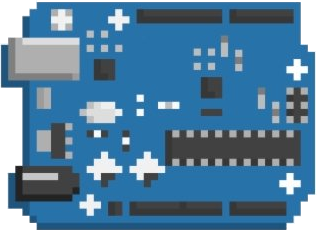
\includegraphics[height=4mm]{Figures/microcontroller_emoji.png}&
  T1 \\ \hline
T2.1 &
  \begin{tabular}[c]{@{}l@{}}\textbf{Reading documentation on the ESP32 collection of libraries}\\ ESP32 has a large amount of features divided between different libraries. \\ Understanding the basic functionalities of the board is essential to \\use all the features in a smart way\end{tabular} &
   10&
   &
   \\ \hline
T2.2 &
  \begin{tabular}[c]{@{}l@{}}\textbf{Reading documentation on TTGO Board}\\ Understand what features the board has and how to use them\end{tabular} &
   5&
   &
   \\ \hline
T2.3 &
  \begin{tabular}[c]{@{}l@{}}\textbf{Reading documentation on PlatformIO}\\ Make sure I follow the most efficient procedures the add-on offers\end{tabular} &
   10&
   &
   \\ \hline
T2.4 &
  \begin{tabular}[c]{@{}l@{}}\textbf{Testing the knowledge aquired}\\ Develop small programs to test all the features that could be useful for the\\research\end{tabular} 	   &
   10&
   
\includegraphics[height=4mm]{Figures/laptop_emoji.png}
   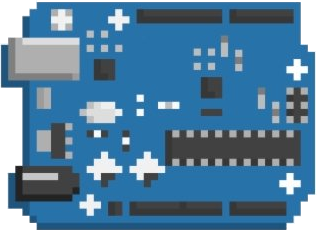
\includegraphics[height=4mm]{Figures/microcontroller_emoji.png}&
  \begin{tabular}[c]{@{}l@{}}T2.1\\ T2.2\\ T2.3\end{tabular} \\ \hline
  \rowcolor[HTML]{C0C0C0}
T3 &
  \textbf{Develop feature rich PoC to make sure I'm ready to start developing} &
   30 &
   
\includegraphics[height=4mm]{Figures/laptop_emoji.png}
   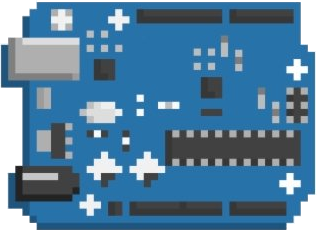
\includegraphics[height=4mm]{Figures/microcontroller_emoji.png}&
  T2 \\ \hline
\end{tabular}%
}
\caption{List of tasks for the Researching and Learning phase}
\label{tab:InitialTasks}
\end{table}


\subsection{Conception and Initiation phase}
% Documentacio preliminar
% Traçar un full de ruta
% Preveure obstacles
% En general copiar lo de l'Aaron
Defining a roadmap is essential to have a well defined project that is easy to manage and complete. This section explains the tasks related to the management and planning of the project in its first stages.\autoref{tab:DocumentationTasks} shows the tasks related as well as its dependencies and resources associated with them: 

\begin{table}[ht]
\centering
\resizebox{\textwidth}{!}{%
\begin{tabular}{|c|l|c|c|c|}
\hline
\rowcolor[HTML]{9B9B9B} 
\textbf{ID} &
  \multicolumn{1}{c|}{\cellcolor[HTML]{9B9B9B}\textbf{Description}} &
  \textbf{\begin{tabular}[c]{@{}c@{}}Work\\ Hours\end{tabular}} &
  \textbf{Resources} &
  \textbf{Deps.} \\ \hline
\rowcolor[HTML]{C0C0C0} 
T4 &
  \begin{tabular}[c]{@{}l@{}}\textbf{Inititial scope}\\ Study the basics of the project and have a good understanding of\\ what sorounds it\end{tabular} &
   26&
   &
  T2 \\ \hline
T4.1   & \begin{tabular}[c]{@{}l@{}}\textbf{Project Context}\\ Define the different topics the project will interact with\end{tabular}                   & 14 &  &    \\ \hline
T4.1.1 & \begin{tabular}[c]{@{}l@{}}\textbf{Academic Context}\\ Define how the research fits into the current academic setting\end{tabular}              & 4 &  &    \\ \hline
T4.1.2 & \begin{tabular}[c]{@{}l@{}}\textbf{Terms and concepts}\\ Define the technologies and resources used in the research\end{tabular}                & 4 &  &    \\ \hline
T4.1.3 & \begin{tabular}[c]{@{}l@{}}\textbf{The problem}\\ Define the problem that wants to be solved by the research\end{tabular}                       & 4 &  &    \\ \hline
T4.1.4 & \begin{tabular}[c]{@{}l@{}}\textbf{Stakeholders}\\ Investigate the actors interested in the research\end{tabular}                               & 2 &  &    \\ \hline
T4.2 &
  \begin{tabular}[c]{@{}l@{}}\textbf{Project Justification}\\ Justify why the research is needed and how it differs from previous ones\end{tabular} &
   2&
   &
  T4.1.3 \\ \hline
T4.3   & \begin{tabular}[c]{@{}l@{}}\textbf{Project Scope}\\ Define what the project is and is not\end{tabular}                                          & 6 &  &    \\ \hline
T4.3.1 & \begin{tabular}[c]{@{}l@{}}\textbf{General Objectives}\\ Define the goals of the research\end{tabular}                                          & 4 &  &    \\ \hline
T4.3.2 & \begin{tabular}[c]{@{}l@{}}\textbf{Risk Assessment}\\ Investigate possible issues that may arise during the course of the research\end{tabular} & 2 &  &    \\ \hline
T4.4   & \begin{tabular}[c]{@{}l@{}}\textbf{Methodology and Rigor}\\ Define methodologies and tools that will help obtain reliable results\end{tabular}  & 4 &  & T2 \\ \hline
T4.4.1 & \begin{tabular}[c]{@{}l@{}}\textbf{Programming workflow}\\ Define the set of procedures that will ensure a bug-free code\end{tabular}             & 2 &  &    \\ \hline
\rowcolor[HTML]{C0C0C0} 
T5 &
  \begin{tabular}[c]{@{}l@{}}\textbf{Review the documentation}\\ Make sure all sections make sense between each other and comment the\\text with the directors\end{tabular} &
   8&
   
\includegraphics[height=4mm]{Figures/teacher_emoji.png}&
  T4 \\ \hline
  \rowcolor[HTML]{C0C0C0} 
T6 &
  \begin{tabular}[c]{@{}l@{}}\textbf{Task analysis}\\ Identify and organize the tasks and subtasks that are going to be part\\of this project\end{tabular} &
   4&
   &
  T5 \\ \hline
  \rowcolor[HTML]{C0C0C0} 
T7 &
  \begin{tabular}[c]{@{}l@{}}\textbf{Project Planning}\\ Estimate the time needed for each task and its dependencies\end{tabular} &
   4&
   &
  T6 \\ \hline
  \rowcolor[HTML]{C0C0C0} 
T8 &
  \begin{tabular}[c]{@{}l@{}}\textbf{Sustainability analysis}\\ Estimate the impact of the project to the environment and society\end{tabular} &
   6&
   &
  T5 \\ \hline
\end{tabular}%
}
\caption{List of tasks for the Conception and Initiation phase}
\label{tab:DocumentationTasks}
\end{table}

\subsection{Design and Implementation phase}
% Convertir el codi a llibreria
% Adaptar la llibreria per tenir acces de lectura a les estructures internes
% Dissenyar estructura del programa
% Implementar mecanisme de sincronitzacio entre nodes
% Implementar la recoleccio de dades
	% Local
	% Internet
% Dissenyar tipus de tests
% Implementar la generacio de tests (Possiblement de forma dinamica)

The first step once there is a clear roadmap is to start preparing the right environment for the experiments, designing and implementing the tools needed. \autoref{tab:ProgramingTasks} shows the tasks related as well as its dependencies and resources associated with them:

The next step after we have a clear roadmap is to set up a good developing environment to speed up code development. In this section we will find some unforeseen circumstances that will delay the implementation.

\begin{table}[ht]
\centering
\resizebox{\textwidth}{!}{%
\begin{tabular}{|c|l|c|c|c|}
\hline
\rowcolor[HTML]{9B9B9B} 
\textbf{ID} &
  \multicolumn{1}{c|}{\cellcolor[HTML]{9B9B9B}\textbf{Description}} &
  \textbf{\begin{tabular}[c]{@{}c@{}}Work\\ Hours\end{tabular}} &
  \textbf{Resources} &
  \textbf{Deps.} \\ \hline
\rowcolor[HTML]{C0C0C0} 
T9 &
  \begin{tabular}[c]{@{}l@{}}\textbf{Make ESP-Prog work on the T-Beam}\\ The documentation was incorrect and the ESP-Prog  needs some additional \\ work to be useful\end{tabular} &
   40&
   	
\includegraphics[height=4mm]{Figures/laptop_emoji.png}
	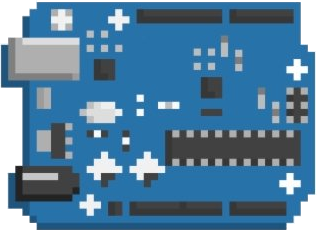
\includegraphics[height=4mm]{Figures/microcontroller_emoji.png}
	
\includegraphics[height=4mm]{Figures/screwdriver_emoji.png}&
  T5 \\ \hline
\rowcolor[HTML]{C0C0C0} 
T10 &
  \begin{tabular}[c]{@{}l@{}}\textbf{Decide which parts of the code are relevant}\\ The PoC is operational but there's bloat that needs to be removed. \end{tabular} &
   20&
   	
\includegraphics[height=4mm]{Figures/laptop_emoji.png}
	
\includegraphics[height=4mm]{Figures/teacher_emoji.png}&
   \\ \hline
\rowcolor[HTML]{C0C0C0} 
T11 &
  \begin{tabular}[c]{@{}l@{}}\textbf{Design library architecture}\\ Research and design a architecture for the library and how its different\\pieces will interact with each other\end{tabular} &
   20&
      
\includegraphics[height=4mm]{Figures/laptop_emoji.png}
&
   T10 \\ \hline
   \rowcolor[HTML]{C0C0C0} 
T12 &
  \begin{tabular}[c]{@{}l@{}}\textbf{Implement library}\\ Implement the library in C++ and make use of OOP\end{tabular} &
   140&
   
\includegraphics[height=4mm]{Figures/laptop_emoji.png}
	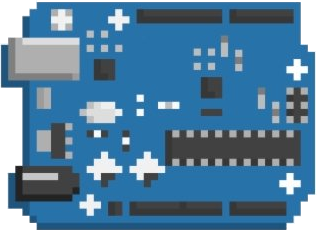
\includegraphics[height=4mm]{Figures/microcontroller_emoji.png}
	
\includegraphics[height=4mm]{Figures/screwdriver_emoji.png}&
   T11\\ \hline
T12.1 &
  \begin{tabular}[c]{@{}l@{}}\textbf{Solve hardware architecture problems}\\ The hardware architecture is more complex than initially thought\end{tabular} &
   40&
   
\includegraphics[height=4mm]{Figures/laptop_emoji.png}
	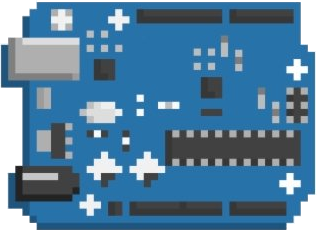
\includegraphics[height=4mm]{Figures/microcontroller_emoji.png}
	
\includegraphics[height=4mm]{Figures/screwdriver_emoji.png}&
   \\ \hline
T12.2 &
  \begin{tabular}[c]{@{}l@{}}\textbf{Solve software issues}\\ FreeRTOS and Radiolib are two complex libraries that require special care\end{tabular} &
   60&
   
\includegraphics[height=4mm]{Figures/laptop_emoji.png}
	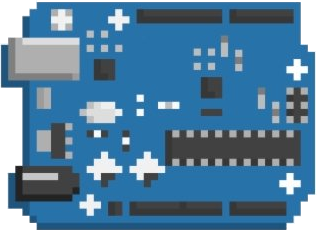
\includegraphics[height=4mm]{Figures/microcontroller_emoji.png}
	
\includegraphics[height=4mm]{Figures/screwdriver_emoji.png}&
   \\ \hline
\rowcolor[HTML]{C0C0C0} 
T13 &
  \begin{tabular}[c]{@{}l@{}}\textbf{Testing}\\ Testing will be conducted through the whole coding process\end{tabular} &
   80&
   	
\includegraphics[height=4mm]{Figures/laptop_emoji.png}
	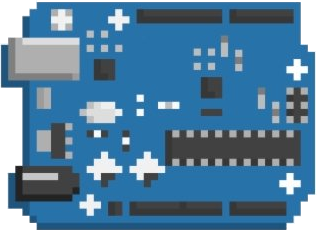
\includegraphics[height=4mm]{Figures/microcontroller_emoji.png}
	
\includegraphics[height=4mm]{Figures/screwdriver_emoji.png}&
  T11 \\ \hline
\end{tabular}%
}
\caption{List of tasks for the Design and Implementation phase}
\label{tab:ProgramingTasks}
\end{table}

% Fer que el ESP-Prog funcioni
% Analitzar llibreria i veure què es queda i què s'enva
% Pensar en la arquitectura de la llibreria
% Passar el codi a C++ i OOP
%% Solucionar problemes amb l'arquitectura (lo de les funcions en instancies)
%% Solucionar problemes de FreeRTOS i RadioLib
% Testing (dir que s'incorpora en les tasques anteriors)






\subsection{Closing phase}
% Documentation wrap up
% Presentation

\autoref{tab:WrapupTasks} shows the tasks related the final stages of the project as well as its dependencies and resources associated with them:

\begin{table}[]
\centering
\resizebox{\textwidth}{!}{%
\begin{tabular}{|c|l|c|c|c|}
\hline
\rowcolor[HTML]{9B9B9B} 
\textbf{ID} &
  \multicolumn{1}{c|}{\cellcolor[HTML]{9B9B9B}\textbf{Description}} &
  \textbf{\begin{tabular}[c]{@{}c@{}}Work\\ Hours\end{tabular}} &
  \textbf{Resources} &
  \textbf{Deps.} \\ \hline
\rowcolor[HTML]{C0C0C0} 
T14 &
  \begin{tabular}[c]{@{}l@{}}\textbf{Documentation wrap up}\\ Make sure the final document is understandable and every \\important topic has been explained in detail. In addition,\\properly format the document and create visual assets\end{tabular} &
   60 &
   
\includegraphics[height=4mm]{Figures/laptop_emoji.png}
   
\includegraphics[height=4mm]{Figures/teacher_emoji.png}&
  T13 \\ \hline
\rowcolor[HTML]{C0C0C0} 
T15 &
  \begin{tabular}[c]{@{}l@{}}\textbf{Presentation}\\ Prepare a visual presentation to show the research to the comitee\end{tabular} &
   40 &
   
\includegraphics[height=4mm]{Figures/laptop_emoji.png}
   
\includegraphics[height=4mm]{Figures/teacher_emoji.png}&
  T14 \\ \hline
\end{tabular}%
}
\caption{List of tasks for the Closing phase}
\label{tab:WrapupTasks}
\end{table}


% Please add the following required packages to your document preamble:
% \usepackage{graphicx}
% \usepackage[table,xcdraw]{xcolor}
% If you use beamer only pass "xcolor=table" option, i.e. \documentclass[xcolor=table]{beamer}
\begin{table}[]
\centering
\resizebox{\textwidth}{!}{%
\begin{tabular}{|c|l|}
\hline
\rowcolor[HTML]{C0C0C0} 
\multicolumn{1}{|l|}{\cellcolor[HTML]{C0C0C0}ID} & Description                                                                 \\ \hline

\includegraphics[height=4mm]{Figures/laptop_emoji.png} & Fully working workstation                                                   \\ \hline
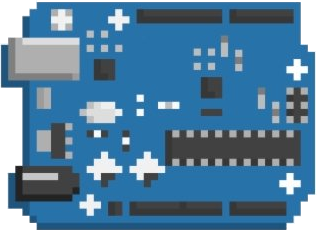
\includegraphics[height=4mm]{Figures/microcontroller_emoji.png}  & TTGO T-Beam board. The amount of boards needed will vary during development \\ \hline

\includegraphics[height=4mm]{Figures/teacher_emoji.png} & The directors of the project. They offer great advice                       \\ \hline

\includegraphics[height=4mm]{Figures/screwdriver_emoji.png} & ESP-Prog. The debugging board. We will only need one                        \\ \hline
\end{tabular}%
}
\caption{Legend of Resources}
\label{tab:Resources}
\end{table}

\subsection{Modifications implications}
Overall, the modifications in the tasks add 18h more of work as the development of the library took way more time than initially planned. The time increase, however, does not make the project impossible to perform in the expected schedule.
%%En total son 461h+18h o 25h/ECTS





